\documentclass[12pt,a4paper]{report}
\setlength\textwidth{145mm}
\setlength\textheight{247mm}
\setlength\oddsidemargin{15mm}
\setlength\evensidemargin{15mm}
\setlength\topmargin{0mm}
\setlength\headsep{0mm}
\setlength\headheight{0mm}
% \openright makes the following text appear on a right-hand page
\let\openright=\clearpage

\input{metadata}

\usepackage[a-2u]{pdfx}

\ifEN\else\usepackage[czech,shorthands=off]{babel}\fi

% See https://en.wikipedia.org/wiki/Canons_of_page_construction before
% modifying the size of printable area. LaTeX defaults are great.
% If you feel it would help anything, you can enlarge the printable area a bit:
%\usepackage[textwidth=390pt,textheight=630pt]{geometry}
% The official recommendation expands the area quite a bit (looks pretty harsh):
% \usepackage[textwidth=145mm,textheight=247mm]{geometry}

%%% TYPICAL FONT CHOICES (uncomment what you like) %%%

% For the "classic" LaTeX fonts (very good for pure math theses), simply
% comment out any other font choices.

% Recommended combo: Libertinus (autoselects Biolinum for sans), typewriter
% font comes from AnonymousPro. If you like libertinus a lot, you can try the
% mono font from Libertinus too -- simply remove the `mono=false` argument.
% `StretchTT=1` seems required to make the PDF/A validation pass.)
\usepackage[mono=false,StretchTT=1]{libertinus}

% IBM Plex font suite: nice, but requires us to fine-tune the sizes and does
% not directly support small caps (\textsc):
%\usepackage[RM={Scale=0.88},SS={Scale=0.88},SScon={Scale=0.88},TT={Scale=0.88},DefaultFeatures={Ligatures=Common}]{plex-otf}

% TeX Gyre combo (Pagella+Heros+Cursor)
%\usepackage{fontspec}
%\setmainfont{TeX Gyre Pagella}
%\setsansfont{TeX Gyre Heros}
%\setmonofont{TeX Gyre Cursor}

% some useful packages
% \usepackage[utf8]{inputenc}
\usepackage{array}
\usepackage[ddmmyyyy]{datetime}
% \usepackage{hyperref}
% \usepackage{float}

\usepackage{microtype} % for better typesetting
\usepackage{amsmath,amsfonts,amsthm,bm}
\usepackage{graphicx}
\usepackage{xcolor}
\usepackage{booktabs}
\usepackage{caption}
\usepackage{floatrow}
% remove this if you won't use fancy verbatim environments
% \usepackage{fancyvrb}

\usepackage{geometry} % for setting custom margins
\usepackage{dcolumn}        % improved alignment of table columns
\usepackage{paralist}       % improved enumerate and itemize

%% Custom packages
\usepackage[htt]{hyphenat} % for breaking long typefont lines in texttt
\usepackage{fvextra} % for breaklines in verbatim environments (extension of fancyvrb)
\usepackage{array} % for fixed column width
\usepackage{multirow} % for borders and merged ranges
\usepackage{soul} % for underlines
\usepackage{geometry} % for setting custom margins
\usepackage{pdflscape} % for landscape pages
\usepackage{tabularx} % for tables (auto width)
\usepackage[export]{adjustbox} % for wide tables/figures
\usepackage{changepage} % for wide tables
\usepackage{float} % for H positioning of tables/figures
\usepackage{dirtytalk} % for quotes using \say
\usepackage{enumitem} % for custom enumeration
% \usepackage{svg} % for SVG images
\usepackage{caption} % for table captions on the top, also for longlisting captions
\usepackage[newfloat, outputdir=.output]{minted} % for code listings

\usepackage{url} % for URLs
\usepackage{xurl} % for long URLs
% hyperref to be included as the last package (except for cleveref and some other packages)
\usepackage{hyperref} % for clickable links
\usepackage{nameref} % for named references
\usepackage[acronym, toc, automake]{glossaries} % for glossaries
\usepackage[para,online,flushleft]{threeparttable} % for table notes

% Bibliography formatting.
% CHECK THE REQUIREMENTS OF YOUR DEPARTMENT AND FACULTY ON THE CITATION FORMAT!
%
% These are relatively "safe" default options that most people use:
\usepackage[natbib,style=numeric,sorting=none]{biblatex}
% alternative with alphanumeric citations (more informative than numbers, and
% more common in computer science journals):
%\usepackage[natbib,style=alphabetic]{biblatex}
%
% ALTERNATIVES THAT CONFORM TO ISO690
% ISO690 is not the greatest citation format ever, but may be formally
% required at Charles University, depending on your faculty and department.
%\usepackage[natbib,style=iso-numeric,sorting=none]{biblatex}
%\usepackage[natbib,style=iso-alphabetic]{biblatex}
% You might want to add extra options such as `maxbibnames=6,maxcitenames=2`
% here to further conform to some of the formatting requirements (see below for
% details). Again, consult your faculty rules.
%
% Additional option choices:
%  - add `giveninits=true` to typeset "E. A. Poe" instead of full Edgar Allan
%  - `terseinits=true` additionaly shortens it to nature-like "Poe EA"
%  - add `maxnames=10` to limit (or loosen) the maximum number of authors in
%    bibliography entry before shortening to `et al.` (useful when referring to
%    book collections that may have hundreds of authors)
%  - use `maxcitenames=2` to finetune the amount of authors listed in text-cite
%    commands (\citet). Corresponding option that only affects the bibliography
%    is `maxbibnames=10`.
%  - `sorting=none` causes the bibliography list to be ordered by the order of
%    citation as they appear in the text, which is usually the desired behavior
%    with numeric citations. Additionally you can use a style like
%    `numeric-comp` that compresses the long lists of citations such as
%    [1,2,3,4,5,6,7,8] to simpler [1--8]. This is especially useful if you plan
%    to add tremendous amounts of citations, as usual in life sciences and
%    bioinformatics.
%  - if you don't like the "In:" appearing in the bibliography, use the
%    extended style (`ext-numeric` or `ext-alphabetic`), and add option
%    `articlein=false`.
%
% possibly reverse the names of the authors with the default styles:
%\DeclareNameAlias{default}{family-given}

% load the file with bibliography entries
\addbibresource{refs.bib}

% remove this if you won't typeset TikZ graphics
\usepackage{tikz}
\usetikzlibrary{positioning} %add libraries as needed (shapes, decorations, ...)

% remove this if you won't typeset any pseudocode
\usepackage{algpseudocode}
\usepackage{algorithm}

% remove this if you won't list any source code
% \usepackage{listings}


\hypersetup{unicode}
\hypersetup{breaklinks=true}

\usepackage[noabbrev]{cleveref}

%%% Some customizations 
% \usemintedstyle{vs} % for Visual Studio Code style
\fvset{breaklines=true, breakanywhere} % for breaklines in verbatim environments
\newenvironment{longlisting}{\captionsetup{type=listing}}{} % for long listings
\definecolor{LightGray}{gray}{0.9} % for listing background color

% Definitions of all glossary/acronym entries
\makeglossaries

% New acronyms

\newacronym{orm}{ORM}{Object-Relational Mapping}

\newacronym{odm}{ODM}{Object-Document Mapping}

\newacronym{ogm}{OGM}{Object-Graph Mapping}

\newacronym{ui}{UI}{User Interface}

\newacronym{llm}{LLM}{Large Language Model}

\newacronym{jit}{JIT}{Just-In-Time}

\newacronym{rest}{REST}{Representational State Transfer}

\newacronym{sse}{SSE}{Server-Sent Events}

\newacronym{ide}{IDE}{Integrated Development Environment}

\newacronym{acp}{ACP}{Agent Client Protocol}

\newacronym{hitl}{HITL}{Human-in-the-Loop}

\newacronym{cot}{CoT}{Chain-of-Thought}

\newacronym{moe}{MoE}{Mixture-of-Experts}

\newacronym{clr}{CLR}{Common Language Runtime}

% From BP

\newacronym{dbms}{DBMS}{Database Management System}

\newacronym{ddl}{DDL}{Data Definition Language}

\newacronym{dml}{DML}{Data Manipulation Language}

\newacronym{sql}{SQL}{Structured Query Language}

\newacronym{rdbms}{RDBMS}{Relational Database Management System}

\newacronym{crud}{CRUD}{Create, Read, Update, Delete}

\newacronym{acid}{ACID}{Atomicity, Consistency, Isolation, Durability}

\newacronym{cte}{CTE}{Common Table Expression}

\newacronym{iot}{IoT}{Internet of Things}

\newacronym{io}{I/O}{Input/Output}

\newacronym{db}{DB}{Database}

\newacronym{cpu}{CPU}{Central Processing Unit}

\newacronym{ram}{RAM}{Random Access Memory}

\newacronym{os}{OS}{Operating System}

\newacronym{ml}{ML}{Machine Learning}

\newacronym{ai}{AI}{Artificial Intelligence}

\newacronym{lpg}{LPG}{Labeled Property Graph}

\newacronym{gdbms}{GDBMS}{Graph Database Management System}

\newacronym{apoc}{APOC}{Awesome Procedures on Cypher}

\newacronym{mmdbms}{MMDBMS}{Multi-Model Database Management System}

\newacronym{api}{API}{Application Programming Interface}

\newacronym{mcp}{MCP}{Model Context Protocol}

\newacronym{ha}{HA}{High Availability}

\newacronym{ft}{FT}{Fault Tolerance}

\newacronym{etl}{ETL}{Extract, Transform, Load}

\newacronym{base}{BASE}{Basically Available, Soft state, Eventually consistent}

\newacronym{ttl}{TTL}{Time To Live}

\newacronym{json}{JSON}{Javascript Object Notation}

\newacronym{csv}{CSV}{Comma Separated Values}

\newacronym{tsv}{TSV}{Tab Separated Values}

\newacronym{uml}{UML}{Unified Modeling Language}

\newacronym{er}{ER}{Entity-Relationship}

\newacronym{cql}{CQL}{Cassandra Query Language}

\newacronym{saas}{SaaS}{Software as a Service}

\newacronym{mql}{MQL}{MongoDB Query Language}

\newacronym{gui}{GUI}{Graphical User Interface}

\newacronym{aql}{AQL}{ArangoDB Query Language}

\newacronym{cli}{CLI}{Command Line Interface}

\newacronym{npm}{NPM}{Node Package Manager}

\newacronym{dnf}{DNF}{Did Not Finish}

\newacronym{rw}{R/W}{Read/Write}


\input{todos} % remove this before compiling the final version

\input{macros} % use this file for various custom definitions


\begin{document}

\include{title}

\tableofcontents

\chapwithtoc{Introduction}

\section*{Motivation}
\label{sec:intro-motivation}

\section*{Goals and Contributions}
\label{sec:intro-goals}

\section*{Results}
\label{sec:intro-results}

\section*{Thesis Outline}
\label{sec:intro-outline}

\include{ch_related}
\chapter{Problem Definition}
\label{chap:problem}

Modern applications rarely talk to their databases directly. Instead, they reach persistent data through an \emph{object-mapping framework} that maps in-memory objects onto an underlying store and exposes a programming-language query interface over it. Depending on the data model, such a framework is called an \ACRfull{orm} for relational databases, an \ACRfull{odm} for document stores, or an \ACRfull{ogm} for graph databases. The mapping framework, together with its entity definitions, mapping configuration, queries, and the surrounding persistence code, constitutes the \emph{persistence layer} of the application.

Over the lifetime of a system, the persistence layer often has to change. A team may move from a relational store to a document or graph database to fit an evolving access pattern, consolidate on a different framework, or target a different language ecosystem entirely. Such a migration is not a mechanical rename: it requires transforming entity definitions, mapping configurations, queries, and framework-specific persistence code, while preserving the externally observable behavior of the application. Because the source and target frameworks may differ in their data models, mapping strategies, query interfaces, and supported features, these transformations are intricate and error-prone.

This thesis designs and implements an \ACRfull{llm}-based assistant that migrates database-layer artifacts across selected ORM, ODM, and OGM frameworks. This chapter states precisely what the assistant is meant to achieve. \Cref{sec:problem-goals} fixes the goals, \cref{sec:problem-nongoals} delimits what is deliberately out of scope, \cref{sec:problem-scope} pins down the concrete frameworks and databases, \cref{sec:problem-example} introduces a running example used throughout the thesis, and \cref{sec:problem-requirements} distills the goals into testable requirements that the evaluation (\cref{chap:evaluation}) revisits.

\section{Goals}
\label{sec:problem-goals}

The overarching goal is an assistant that, given the database-layer artifacts of an application written against a \emph{source} framework, produces the equivalent artifacts for a chosen \emph{target} framework, and does so with an \emph{execution-grounded correctness guarantee} rather than mere syntactic plausibility. Concretely, the thesis pursues four goals.

\begin{description}
  \item[G1 -- Translation across paradigms.] Translate the persistence-layer artifacts of a source \acrshort{orm} into the equivalent artifacts of a target \acrshort{odm} or \acrshort{ogm}, crossing the relational/document and relational/graph boundaries. The unit of translation is twofold: \emph{schema} (entity classes and their mapping configuration) and \emph{queries} (the framework-specific query methods), independently or together.

  \item[G2 -- Correctness by Execution.] A translation is only surfaced to the user after it has been compiled with the real target toolchain (i.e. \ACRfull{cli} tools and language-specific libraries) and executed against a live database, and after the data it returns has been checked for semantic and logical equivalence\footnote{Logically equivalent queries output semantically and quantitatively the same result sets with same primitive values (i.e. with comparable data types and same values given differences in the underlying data stores) but in different data formats, e.g. \acrshort{csv} tables vs. \acrshort{json} documents, but in context of ORM/ODM/OGM frameworks we should get similar instances (i.e. logically equivalent properties) of entities in supported languages (e.g. C\# objects vs. Java objects)} with the data returned by the source. (see \cref{chap:validation}).~\cite{execoder2025}

  \item[G3 -- Generality.] Cover a space wide enough to show that the approach is not tied to a single pair of frameworks: three structurally different source query dialects (LINQ, raw SQL, and HQL) and two distinct non-relational paradigms (document and graph). Adding a framework should be a mechanical extension of the engine, not a redesign of the approach (\cref{chap:design}).

  \item[G4 -- Usability and Observability.] Deliver the assistant as an interactive \acrlong{ui}, in which a user submits source artifacts, watches the translation proceed step by step, inspects every intermediate result, and intervenes when necessary. Every run is fully traced and reproducible.
  
  \item[G5 -- Experimental Evaluation.] Demonstrate that the assistant meets the above goals through a systematic evaluation (\cref{chap:evaluation}) that measures correctness, robustness, and the amount of human intervention required through quantitative and statistical metrics.
\end{description}

Note that, the construction of the theoretical background for the assistant and its experimental validation are the subject of this thesis; the implementation itself was first delivered as a research project implemented by the author of this thesis within the Adaptive Data Management (ADaM) research group, and it builds on the rule-based \emph{ORMorpher} line of work \cite{abrahamORMorpherInteractiveFramework2026, abrahamFrameworkAgnosticQueryAdaptation2025}. \Cref{chap:related} positions the thesis against that background.

\section{Non-Goals}
\label{sec:problem-nongoals}

Equally important is what the assistant is \emph{not} expected to do. Stating non-goals explicitly keeps the contribution well-defined and prevents the reader from measuring the work against problems it never set out to solve.

\begin{description}
  \label{item:non-goal-n1} \item[N1 -- Not a data-migration (\acrshort{etl}) tool.] The assistant translates \emph{code} (schema and queries), not the data itself. Populating logically equivalent target databases from the relational source is a separate, one-time, semi-automatic step performed with established \Acrfull{etl} tooling (MongoDB Relational Migrator~\cite{mongo-rel-migrator} and the Neo4j ETL Tool~\cite{neo4j-etl-tool}); it is a precondition for validation, not part of the translation pipeline. \todo{referene the \cref{chap:architecture} when available.}

  \item[N2 -- Not a performance optimizer.] The assistant aims at \emph{correct}, idiomatic translations, not at selecting the fastest target framework or tuning the generated queries. Performance-aware framework \emph{selection} is the province of the complementary ILP-based advisor in the ORMorpher line \cite{abrahamUnifiedFrameworkORM} and is left to future work (\cref{chap:future}).\todo{add more works from the research group}

  \item[N3 -- Not a general-purpose code translator.] The scope is the persistence layer. Business logic, presentation code, and application wiring outside the data-access layer are not translated.
  
  \item[N3 -- Not a general-purpose assistant.] The assistant is a semi-deterministic graph that does not allow arbitrary user prompts. Unlike general-purpose coding assistants, such as Claude Code\footnote{\url{https://code.claude.com/docs/en/overview}}, GitHub Copilot\footnote{\url{https://docs.github.com/en/copilot}}, or general-purpose chatbots, such as OpenAI ChatGPT (\footnote{\url{https://chatgpt.com/}}), Google Gemini\footnote{\url{https://gemini.google.com/}}, the initial prompt and its format have to be specific, and the user can only intervene at the end of a constant number of self-corrected translation attempts.

  \item[N4 -- Bounded automation, not full autonomy.] When automated repair fails within a bounded number of attempts, the system deliberately pauses and hands control to a human rather than retrying indefinitely or guessing. A fully autonomous, open-ended agent is not a goal of this thesis (the rationale is given in \cref{chap:design}).

  \item[N5 -- A fixed, curated set of frameworks and versions.] The assistant targets specific, pinned framework versions (\cref{sec:problem-scope}) rather than arbitrary or legacy ones. This is what makes grounded, compile-against-the-real-API generation possible.
\end{description}

\section{Scope: Frameworks, Databases, and Versions}
\label{sec:problem-scope}

The assistant translates from three .NET relational source frameworks into two Java Spring Data non-relational targets (as part of Spring Boot\footnote{\url{https://spring.io/projects/spring-boot}} ecosystem). The source side covers the three dominant access styles in the .NET ecosystem: a full ORM with LINQ\footnote{\url{https://learn.microsoft.com/en-us/dotnet/csharp/linq/}} (Entity Framework Core), a mature ORM with its own query language (NHibernate with LINQ\footnote{\url{https://nhibernate.info/doc/nhibernate-reference/querylinq.html}} or HQL\footnote{\url{https://nhibernate.info/doc/nhibernate-reference/queryhql.html}}), and a thin micro-ORM over raw SQL~\cite{kalecheva-ansi-2023-standard} (Dapper). The target side covers the two principal non-relational paradigms: document-based (Spring Data MongoDB) and graph-based (Spring Data Neo4j) submodules of the Spring Data module. \Cref{tab:scope} summarizes the supported frameworks, their data models, query interfaces, and the pinned versions used throughout the thesis.

\begin{table}[t]
\centering
\caption{Supported frameworks, data models, query interfaces, and pinned versions. The source frameworks run on .NET~10; the target frameworks on Java~25 / Spring~Boot~4.0.}
\label{tab:scope}
\resizebox{\columnwidth}{!}{%
\begin{tabular}{@{}lllll@{}}
\toprule
Role & Framework & Paradigm & Query interface & Version \\
\midrule
Source & Entity Framework Core & ORM (relational)   & LINQ              & 10  \\
Source & NHibernate            & ORM (relational)   & HQL               & 5.5 \\
Source & Dapper                & micro-ORM (relational) & raw SQL       & 2.1 \\
Target & Spring Data MongoDB   & ODM (document)     & Query/Criteria\footnote{\url{https://docs.spring.io/spring-data/mongodb/reference/5.0/mongodb/template-query-operations.html}}, Aggregation\footnote{\url{https://docs.spring.io/spring-data/mongodb/reference/5.0/mongodb/aggregation-framework.html}} & 5.0 \\
Target & Spring Data Neo4j     & OGM (graph)        & Cypher-DSL\footnote{\url{https://neo4j.github.io/cypher-dsl/2025.3.0/}}        & 8.1 \\
\bottomrule
\end{tabular}
}
\end{table}

The relational source is a Microsoft SQL Server~2022 instance pre-loaded with the \emph{WideWorldImporters} sample database \cite{wideWorldImporters}; the document and graph targets are MongoDB~8.2.6\footnote{\url{https://www.mongodb.com/docs/v8.2/}} and Neo4j~2026.02.2\footnote{\url{https://neo4j.com/docs/}}, populated with logically equivalent data through the one-time ETL step (\hyperref[item:non-goal-n1]{N1}). The ETL process uses heuristics based on primary, foreign key relationships, number of attributes, and more. The complete information about the ETL processes can be found in their respective documentation (see footnotes). 
Fixing the versions is a deliberate design choice: because the exact target API is known, the assistant can generate code against the real dependency manifest (a pinned \texttt{.csproj} or \texttt{pom.xml}) instead of relying on the language model's recollection of an API surface that changes between releases (\cref{chap:prompting}).

\section{Running Example}
\label{sec:problem-example}

To make the problem concrete -- and to provide a thread that recurs through the workflow (\cref{chap:workflow}), prompting (\cref{chap:prompting}), and validation (\cref{chap:validation}) chapters -- we introduce a single small example: one entity and one query, migrated from Entity Framework Core to Spring Data MongoDB. Even at this minimal size the migration already requires genuine modelling decisions.

\subsection{Input: the source artifacts}

\Cref{lst:ex-source-schema} shows the source \emph{schema}: a \texttt{Customer} entity in Entity Framework Core, mapped to a relational table and holding a one-to-many association to its orders by foreign key. \Cref{lst:ex-source-query} shows the source \emph{query}, expressed in LINQ: all customers that have at least one order placed after a cut-off date.

\begin{listing}[t]
\begin{minted}[linenos, breaklines, frame=single]{csharp}
[Table("Customers", Schema = "Sales")]
public class Customer
{
    [Key]
    public int CustomerID { get; set; }
    public required string CustomerName { get; set; }
    public ICollection<Order> Orders { get; set; }
}
\end{minted}
\caption{Source schema -- an Entity Framework Core entity (LINQ source dialect).}
\label{lst:ex-source-schema}
\end{listing}

\begin{listing}[t]
\begin{minted}[linenos, breaklines, frame=single]{csharp}
// Customers with at least one order placed after a cut-off date.
db.Customers
  .Where(c => c.Orders.Any(o => o.Date > cutoff));
\end{minted}
\caption{Source query -- a LINQ expression over the entity of \cref{lst:ex-source-schema}.}
\label{lst:ex-source-query}
\end{listing}

\subsection{Output: the target artifacts}

\Cref{lst:ex-target-schema} shows the translated \emph{schema} in Spring Data MongoDB. The relational table becomes a \texttt{@Document} collection, the integer primary key is mapped to the document identifier, and -- crucially -- the foreign-key association must be modelled explicitly as either an \emph{embedded} sub-document or a \emph{reference}. The two choices lead to materially different documents and to different queries with different performance and memory characteristics; here the orders are kept as a reference. \Cref{lst:ex-target-query} shows the translated \emph{query}: the LINQ \texttt{\.Any} over a navigation property becomes a MongoDB aggregation pipeline that joins the referenced collection and matches on the date, and must return the same customers as the source.

\begin{listing}[t]
\begin{minted}[linenos, breaklines, frame=single]{java}
@Document("customers")
class Customer {
    @Id String id;
    String customerName;
    @DocumentReference List<Order> orders;
}
\end{minted}
\caption{Target schema -- a Spring Data MongoDB document. The foreign-key association becomes an explicit reference (the embed-versus-reference decision is a real modelling choice).}
\label{lst:ex-target-schema}
\end{listing}

\begin{listing}[t]
\begin{minted}[linenos, breaklines, frame=single]{java}
// Equivalent MongoDB query using the aggregation pipeline.
var agg = Aggregation.newAggregation(
    Aggregation.lookup("orders", "orders", "_id", "orders"),
    Aggregation.match(Criteria.where("orders.date").gt(cutoff))
);
mongoTemplate
    .aggregate(agg, "customers", Customer.class)
    .getMappedResults();
\end{minted}
\caption{Target query -- the LINQ expression of \cref{lst:ex-source-query} as an equivalent MongoDB aggregation pipeline.}
\label{lst:ex-target-query}
\end{listing}

\subsection{Why even this is non-trivial}

\Cref{fig:paradigm-mapping} makes the data-model mismatch concrete: the same \texttt{Customers}/\texttt{Orders} foreign-key association has no one-to-one image in either target paradigm. This example exhibits, in miniature, every difficulty the assistant must handle. The data models do not align one-to-one: a foreign-keyed table is neither a document nor a graph, so the translator must \emph{decide} how to represent the association.

\begin{figure}[ht]
\centering
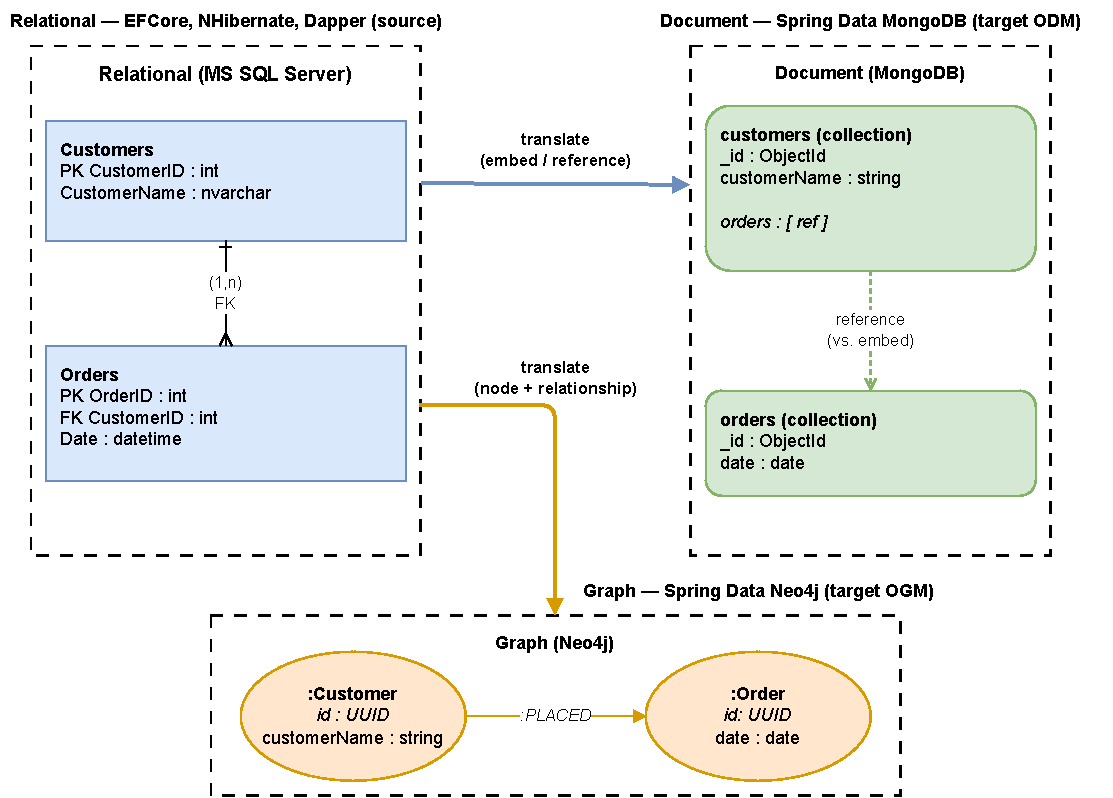
\includegraphics[width=\linewidth]{img/uom_paradigm_mapping.pdf}
\caption{The same relational association translated into the two target models. The document model must choose between embedding and referencing the orders; the graph model turns the entities into nodes joined by a typed relationship.}
\label{fig:paradigm-mapping}
\end{figure} 

Types must be remapped (the integer key becomes a string document identifier). The query must be rewritten into a different idiom (a relational navigation becomes a document aggregation) while returning logically the same result set -- code that merely compiles is not enough. A realistic application multiplies this by dozens of entities and hundreds of queries, each carrying a small decision that can silently break correctness. This is precisely the slow, manual, risky work the assistant is meant to automate \emph{and} verify.

\section{Requirements}
\label{sec:problem-requirements}

The goals of \cref{sec:problem-goals} translate into four properties that a translation produced by the assistant must satisfy. These are the criteria against which the approach is evaluated in \cref{chap:evaluation}.

\begin{description}
  \label{desc:requirements-r1} \item[R1 -- Transformation correctness.] The translated schema and query must be syntactically valid and must compile against the pinned target toolchain. Non-compiling output is rejected before it can reach the user.

  \label{desc:requirements-r2} \item[R2 -- Semantic preservation.] When executed against a live target database holding logically equivalent data, the translated query must return logically the same data as the source query, up to differences that are provably harmless (e.g. field ordering, floating-point precision, or a deterministic reversal of sort order). Equivalence is established by structural comparison of the execution results, not by inspection of the code (\cref{chap:validation}).

  \label{desc:requirements-r3} \item[R3 -- Robustness.] The system must recover from the typical failure modes of language-model code generation -- hallucinated APIs, type mismatches, malformed structured output -- through bounded, automated self-repair, and must degrade gracefully (a controlled hand-off to a human) when repair does not converge.

  \label{desc:requirements-r4} \item[R4 -- Minimal manual intervention.] A correct translation should require as little human effort as possible. The amount of required intervention -- measured as the fraction of runs that reach the human-handoff state -- is a key metric in the evaluation.
\end{description}

Requirements \hyperref[desc:requirements-r1]{R1} and \hyperref[desc:requirements-r2]{R2} are objective, machine-checkable correctness conditions; \hyperref[desc:requirements-r3]{R3} and \hyperref[desc:requirements-r4]{R4} concern the assistant's behaviour around the inevitable cases where the model's first attempt is wrong. The remainder of the thesis shows how the workflow (\cref{chap:workflow}), the orchestration design (\cref{chap:design}), the validation machinery (\cref{chap:validation}), and the prompting strategy (\cref{chap:prompting}) together make these requirements achievable.

\include{ch_overhead}
\chapter{The Translation Workflow}
\label{chap:workflow}

\section{High-Level View}
\label{sec:workflow-overview}

\section{A trace of a running example}
\label{sec:workflow-trace}

\chapter{Design Decisions and Orchestration}
\label{chap:design}

\chapter{Correctness, Validation, and Equivalence}
\label{chap:validation}

\chapter{Prompt and Context Engineering}
\label{chap:prompting}

\chapter{Authoring Migration Inputs}
\label{chap:input}

\chapter{Architecture and Implementation}
\label{chap:architecture}

\include{ch_evaluation}
\include{conclusion}
\include{ch_future}
\include{bibliography}


%%% Figures used in the thesis (consider if this is needed)
\listoffigures

%%% Tables used in the thesis (consider if this is needed)
%%% In mathematical theses, it could be better to move the list of tables to the beginning of the thesis.
\listoftables

%%% Listings used in the thesis (consider if this is needed)
\listoflistings

%%% Abbreviations used in the thesis, if any, including their explanation
%%% In mathematical theses, it could be better to move the list of abbreviations to the beginning of the thesis.
\printglossary[type=\acronymtype, title=List of Abbreviations, toctitle=List of Abbreviations]

\printglossary

\appendix
\chapter{Prompt Context Snippets}
\label{chap:appendix-context-snippets}

This chapter contains the context snippets that were used to prompt the language model for generating the code translations. The snippets are organized by the type of context they provide, such as sandbox configuration files (i.e. build tool configurations) in \cref{sec:appendix-sandbox-config}, schema definitions, query examples, and other relevant code fragments.

\section{Sandbox Configuration Files}
\label{sec:appendix-sandbox-config}

\begin{listing}[H]
\inputminted[fontsize=\footnotesize, linenos, breaklines, frame=single]{xml}{code/efcore-sandbox.csproj}
\caption{Entity Framework Core 8.0.0 \texttt{.csproj} file for the .NET sandbox project.}
\label{lst:efcore-sandbox-csproj}
\end{listing}

\begin{listing}[H]
\inputminted[fontsize=\footnotesize, linenos, breaklines, frame=single]{xml}{code/nhibernate-sandbox.csproj}
\caption{NHibernate \texttt{.csproj} file for the .NET sandbox project.}
\label{lst:nhibernate-sandbox-csproj}
\end{listing}

\begin{listing}[H]
\inputminted[fontsize=\footnotesize, linenos, breaklines, frame=single]{xml}{code/dapper-sandbox.csproj}
\caption{Dapper \texttt{.csproj} file for the .NET sandbox project.}
\label{lst:dapper-sandbox-csproj}
\end{listing}

\begin{listing}[H]
\inputminted[fontsize=\footnotesize, linenos, breaklines, frame=single]{xml}{code/mongo-pom.xml}
\caption{MongoDB \texttt{pom.xml} file for the Java sandbox project.}
\label{lst:mongo-pom-xml}
\end{listing}

\begin{listing}[H]
\inputminted[fontsize=\footnotesize, linenos, breaklines, frame=single]{xml}{code/neo4j-pom.xml}
\caption{Neo4j \texttt{pom.xml} file for the Java sandbox project.}
\label{lst:neo4j-pom-xml}
\end{listing}


% if your attachments are complicated, describe them in a separate appendix
%\chapter{Supplementary Material from the Implementation}
\label{app:implementation}

This appendix collects the concrete, verbatim artifacts referenced from the main
text. They are reproduced from the Universal Object Mapping
repository~\cite{corovcakUOMRepository2026} and are intended as a reference for the
reader who wishes to inspect the exact inputs, schemas, and outputs behind the
workflow described in \cref{chap:workflow}.

\section{Structured-Output and Tool Schemas}
\label{app:pydantic-schemas}

The typed interfaces through which model output re-enters the graph state
(\cref{sec:prompting-structured}) are defined as Pydantic models; the listings below
reproduce their fields with abbreviated descriptions.

\Cref{lst:app-extraction} shows the extraction schema. The code fields accept a
list of strings (one per line) so that the original indentation survives the
provider's JSON transport, and are joined back into a single string by a
post-validation hook; the \texttt{error} field lets the model report an unfulfillable
request as data (\cref{sec:workflow-extract}).

\begin{listing}[H]
\begin{minted}[linenos, breaklines, fontsize=\small, frame=single]{python}
class ExtractionOutput(BaseModel):
    source_schema_code: list[str] | str | None   # source schema, line by line
    source_query_code:  list[str] | str | None   # source queries, line by line
    translation_type:   TranslationType          # SCHEMA | QUERY | BOTH
    source_target:      FrameworkEnum            # identified origin framework
    source_target_version:      str | None
    destination_target: FrameworkEnum            # identified target framework
    destination_target_version: str | None
    error: str | None = None   # set when the request cannot be fulfilled

    @model_validator(mode="after")
    def join_lists(self): ...   # joins list-form code fields into strings
\end{minted}
\caption{The extraction schema (abridged from \texttt{react\_agent/graph.py}).}
\label{lst:app-extraction}
\end{listing}

\Cref{lst:app-save-tool} shows the argument schema of the single state-writing
\texttt{save\_translation} tool that replaced monolithic structured output for the
generation stage (\cref{sec:prompting-structured}). The two body fields carry only the
region below the harness seam; the entry-point class names are baked into the argument
descriptions and are no longer the model's responsibility.

\begin{listing}[H]
\begin{minted}[linenos, breaklines, fontsize=\small, frame=single]{python}
def build_save_translation_tool(translation_type, source_entry, target_entry):
    # args schema (both fields required, descriptions abridged):
    #   source_validation_body: str
    #     "SOURCE-side harness BODY: entity classes, query classes, and the
    #      entrypoint class named exactly `{source_entry}`. No imports, no
    #      redeclaration of injected serializer/runtime/factory classes."
    #   target_validation_body: str
    #     "TARGET-side harness BODY ... entrypoint named exactly `{target_entry}`."
    # The tool persists the fields to state via Command(update=...) and is to be
    # called EXACTLY ONCE at the end of the agent's run.
\end{minted}
\caption{The \texttt{save\_translation} tool contract (abridged from \texttt{react\_agent/translation\_draft.py}).}
\label{lst:app-save-tool}
\end{listing}

\Cref{lst:app-verdicts} shows the two verdict schemas: the judge's structured output
(\cref{sec:validation-judge}) and the resume payload of the human-intervention
interrupt (\cref{sec:workflow-human}), which deliberately mirror each other so that a
human decision re-enters the loop through the same shape as an automated one.

\begin{listing}[H]
\begin{minted}[linenos, breaklines, fontsize=\small, frame=single]{python}
class EvaluationOutput(BaseModel):
    decision: Literal["ACCEPT", "REJECT"]
    explanation: str          # mandatory; becomes the repair feedback

class HumanInterventionResponse(BaseModel):
    decision: Literal["accept", "reject"]
    feedback: str             # targeted correction pointers on reject
\end{minted}
\caption{The judge and human-intervention verdict schemas.}
\label{lst:app-verdicts}
\end{listing}

\section{Per-Node System Prompts}
\label{app:system-prompts}

The prompts below are reproduced from \texttt{react\_agent/prompts.py}
(\cref{chap:prompting}). Placeholders in braces are interpolated at run time.

\subsection*{Input extraction}

\begin{longlisting}
\begin{minted}[breaklines, fontsize=\small, frame=single]{text}
You are an information extractor. Your goal is to extract source schema code, source query code, origin framework/version, destination framework/version, and translation type from the user's messages.

Allowed origin frameworks: {origin_frameworks}
Allowed destination frameworks: {destination_frameworks}

Extraction rules:
1. You must identify the origin framework and the destination framework from the user's messages.
2. You must identify IF the code is a schema (entities/models+context/sessions/configs, etc.) or a query for the given origin framework, or both.
3. If some data has already been extracted, you must use it as is and only extract the missing data.
4. Output specific structured outputs exactly as requested. Do not provide markdown wrapping if native tools capture the output natively.
5. Keep source_schema_code and source_query_code as raw code snippets when available.
6. Preserve the original formatting (including indentation and line breaks) of the extracted code snippets.
\end{minted}
\caption{System prompt of the input-extraction stage.}
\label{lst:app-prompt-extraction}
\end{longlisting}

\subsection*{Schema inspection}

\begin{longlisting}
\begin{minted}[breaklines, fontsize=\small, frame=single]{text}
You are a database schema inspector. Your goal is to examine source and target database schemas to provide context for code translation.

You have access to database tools that can:
- List collections/tables/node labels/relationship types in databases
- Inspect schema structures (columns, fields, nodes, relationships/edges)
- Sample documents/rows/nodes/edges to understand data shapes

Your task:
1. Inspect the SOURCE database schema relevant to the code being translated.
   - For MS SQL: use the prebuilt mssql tools to list tables, describe columns, and sample rows.
   - For MongoDB: use mongodb tools to list collections, inspect document schemas, and sample documents.
   - For Neo4j: use the prebuilt neo4j tools to list node labels, relationship types, and sample nodes/edges.
2. Inspect the TARGET database schema if applicable (e.g., if translating from SQL to MongoDB, inspect what MongoDB collections exist).
3. Focus on ONLY the entities/models/relationships and their relationships relevant to the code being translated.
4. Return a concise but complete summary of the relevant source and target schemas. Do not include a preamble or postamble. The summary will become part of the system prompt for another LLM agent that will perform the actual code translation.

System time: {system_time}
\end{minted}
\caption{System prompt of the schema-inspection stage.}
\label{lst:app-prompt-inspector}
\end{longlisting}

\subsection*{Translation generation}

The generation prompt is assembled dynamically per framework pair
(\cref{sec:prompting-grounding}); the invariant contract is reproduced below, with the
interpolated blocks -- the pinned manifests, the worked mapping examples, and the
harness body-structure references -- elided for space.

\begin{longlisting}
\begin{minted}[breaklines, fontsize=\small, frame=single]{text}
You are a Universal Object Mapping architect. Your goal is to aid in translating database schema structures and query logic between diverse languages and frameworks.

Source Framework: {source_target}
Destination Framework: {destination_target}

Core translation contract:
1. Identify whether the user input contains schema code, query code, or both.
2. Translate only what is requested by translation type.
3. Preserve behavior, field intent, and query semantics.
4. Keep translated query methods semantically equivalent to the source query method. Do not introduce synthetic validator parameters (for example sortByField/ascending) unless they already exist in source query code.
5. Keep schema code and query code separated.
6. CRITICAL - translate ONLY what the user provided. Translate exclusively the entities and fields present in the user's <source_schema_code> and the queries in <source_query_code>. NEVER introduce an entity, field, or query that is not in the user's input. The examples below demonstrate STRUCTURE ONLY [...]
7. You finish by calling the single `save_translation` tool EXACTLY ONCE with every required field filled. There is no separate JSON output. [...]
8. The `*_validation_body` fields are the RUNNABLE harness body ONLY: start directly at the schema/entity declarations, then the query classes, then the entrypoint class with `main`/`Main` that validates each entity and runs each query. The fixed boilerplate - `import`/`using`/`package`/`namespace` lines, the JSON serializer, the runtime-support and DB template-factory classes - is INJECTED FOR YOU around your body. Do NOT write those lines and do NOT redeclare those classes.
   - source_validation_body MUST declare the source entrypoint class named exactly `{source_entry}`.
   - target_validation_body MUST declare the target entrypoint class named exactly `{target_entry}`.
9. All code must be properly indented with real line breaks. DO NOT wrap field values in XML tags or markdown code fences. DO NOT use comments or placeholders in code - it WILL be executed. Never save null or empty values.

Framework rules:
1. For Java schema classes, avoid public access modifier unless explicitly required.
2. For Spring Data MongoDB queries, use MongoTemplate with Query/Criteria API.
3. For Spring Data Neo4j queries, use Neo4jTemplate and Cypher-DSL (Statement-based), not raw string concatenation.
4. Keep translated query method shape close to source query method shape. [...]

Additional rules:
1. You do NOT run validators or compile code. After you call `save_translation`, the translated code is assembled with the canonical prelude and validated automatically by a downstream pipeline (compile + run on both sides, then equivalence). If it fails, you will be re-invoked with concrete feedback to fix and re-save. [...]
2. You have research tools - use them to get the exact API right before saving:
   - Use `search_spring_docs` to query the Spring documentation [...]
   - Use `microsoft_docs_search`, `microsoft_code_sample_search`, and `microsoft_docs_fetch` for Microsoft documentation and code samples.
   - Use `search` to query the web [...]

--- Validation setup configuration ---
[pinned .csproj of the source framework and pom.xml of the target framework]

--- TARGET-LANGUAGE MAPPING REFERENCE ---
[worked input/output mapping examples for the framework pair, structure only]

--- VALIDATION BODY STRUCTURE REFERENCE ---
[the region of each canonical harness snippet below the seam marker]
\end{minted}
\caption{Partial system prompt of the translation-generation stage.}
\label{lst:app-prompt-generation}
\end{longlisting}

\subsection*{Finalization}

\begin{longlisting}
\begin{minted}[breaklines, fontsize=\small, frame=single]{text}
You are a Universal Object Mapping finalizer.

A translation has just been VALIDATED end-to-end: the harness you are given compiled, executed against the database, and passed semantic equivalence against the source. The translation is already CORRECT. Your job is NOT to translate. Your job is to EXTRACT the clean, production-ready target code from the validated harness, removing only the validation scaffolding.

Hard rules:
1. SOURCE OF TRUTH is the validated harness. Copy the entity definitions and the query logic VERBATIM from it. Do NOT re-translate, rename, reorder fields, or change any query predicate, filter, projection, sort, or aggregation - those exact semantics are what equivalence verified.
2. REMOVE only validation-only scaffolding:
   - the JSON serializer class, the runtime-support class, the template/context/db factory class, logging setup, and their imports.
   - the entrypoint class's main/Main method, validate*/ValidateEntity methods, and all results-collection / JSON-writing / env-path code.
   - per-query validation helpers (harness()/RunQuery, count/firstSample/lastSample, and deterministic ORDER BY / Sort / limit / skip that exist ONLY to make validation deterministic and were not in the user's original query).
   - JSON-serialization annotations that are not part of the object mapping (e.g. [JsonPropertyName], @JsonIgnoreProperties, @ReadOnlyProperty added for validation). KEEP genuine ORM mapping annotations: @Document, @Field, @Id, @Node, @Property, @DocumentReference, [Table], [Key], [ForeignKey], [Column], etc.
3. KEEP the genuine production code: the entity/model classes with their ORM mapping, and the production query method(s) carrying the exact validated predicate. Place the queries in a single clean query class with one method per source query, named to match the source (query1..queryN / Query1..QueryN), each returning the production result (not the validation metadata map).
4. Include the minimal imports needed for the production code to compile. [...]
5. Emit CANONICAL, STABLE structure - this code is compared across runs with a CodeBleu (AST + data-flow) metric, so structure must be deterministic: entities in the same declaration order as the validated harness (one class per entity), then the query class with methods in source order. Consistent 4-space indentation. No comments, no markdown code fences, no prose, no placeholders.
\end{minted}
\caption{System prompt of the finalization stage (abridged).}
\label{lst:app-prompt-finalize}
\end{longlisting}

The judge's prompt (\cref{sec:validation-judge}) is a short instruction constructed
inline: it wraps the recent validation outputs in a \texttt{<validation\_results>}
block and asks, \emph{``Is the translation logically equivalent and syntactically
valid? Provide your reasoning and output ACCEPT or REJECT,''} with the response bound
to the \texttt{EvaluationOutput} schema of \cref{lst:app-verdicts}.

\section{Contextual Validation Harness Snippets}
\label{app:snippets}

Each framework contributes two contextual snippets -- a schema-validation and a
query-execution entry point -- split by the marker
\mintinline{text}{// --- Schema and Related Settings ---} into the invariant prelude
that the harness assembler injects and the body region whose \emph{structure} the
model imitates (\cref{sec:validation-grounding}). \Cref{tab:app-snippets} lists the
files and their deterministic entry-point class names.

\begin{table}[H]
\centering
\caption{Contextual snippet files and entry-point class names per framework.}
\label{tab:app-snippets}
\small
\begin{tabular}{@{}l l l@{}}
\toprule
\textbf{Framework} & \textbf{Schema validation} & \textbf{Query execution} \\
\midrule
EF Core & \texttt{EFCoreSchemaValidationEntrypoint} & \texttt{EFCoreQueryEntrypoint} \\
Dapper & \texttt{DapperSchemaValidationEntrypoint} & \texttt{DapperQueryEntrypoint} \\
NHibernate & \texttt{NHibernateSchemaValidationEntrypoint} & \texttt{NHibernateQueryEntrypoint} \\
Spring Data MongoDB & \texttt{MongoSchemaValidationEntrypoint} & \texttt{MongoQueryEntrypoint} \\
Spring Data Neo4j & \texttt{Neo4jSchemaValidationEntrypoint} & \texttt{Neo4jQueryEntrypoint} \\
\bottomrule
\end{tabular}
\end{table}

\Cref{lst:app-serializer-cs} reproduces the core of the invariant .NET prelude: the
serializer configuration that realizes the serialization contract of
\cref{sec:validation-equivalence}. The Java prelude enforces the same rules through
Jackson (ISO-8601 UTC timestamps at millisecond precision,
\texttt{BigDecimal.setScale(3, HALF\_UP)}, alphabetical property and map-key ordering).

\begin{listing}[H]
\begin{minted}[linenos, breaklines, fontsize=\small, frame=single]{csharp}
public static readonly JsonSerializerOptions Options = new()
{
    PropertyNamingPolicy = new CustomCamelCaseNamingPolicy(),   // CustomerID -> customerId
    DictionaryKeyPolicy  = new CustomCamelCaseNamingPolicy(),
    DefaultIgnoreCondition = JsonIgnoreCondition.Never,
    ReferenceHandler = ReferenceHandler.IgnoreCycles,
    TypeInfoResolver = new DefaultJsonTypeInfoResolver
        { Modifiers = { AlphabetizeProperties() } },            // fixed field order
    Converters = {
        new StrictIsoDateTimeConverter(),        // yyyy-MM-dd'T'HH:mm:ss.fff'Z', UTC
        new StrictIsoDateTimeOffsetConverter(),
        new FixedDecimalConverter(),             // "0.000" fixed 3-decimal scale
        new FixedDoubleConverter(),
        new JsonStringEnumConverter(new CustomCamelCaseNamingPolicy())
    }
};
\end{minted}
\caption{The invariant .NET serializer configuration (from \texttt{EFCoreQueryEntrypoint.cs}); the Java prelude mirrors every rule in Jackson.}
\label{lst:app-serializer-cs}
\end{listing}

\Cref{lst:app-runquery} shows the per-query digest producer that every query harness
uses: each query is reduced to its count and its two boundary samples under a
deterministic ordering, keyed \texttt{query1..queryN} in the results JSON that the
equivalence check of \cref{sec:validation-equivalence} consumes.

\begin{listing}[H]
\begin{minted}[linenos, breaklines, fontsize=\small, frame=single]{csharp}
private static object RunQuery<T>(Func<IQueryable<T>> q,
                                  Func<T, object>? orderBySelector = null)
{
    var query = q();
    var count = query.Count();
    return new {
        sqlString = query.ToQueryString(), count,
        firstSample = count > 0
            ? (orderBySelector != null
                ? q().OrderBy(orderBySelector).FirstOrDefault()
                : query.FirstOrDefault()) : default,
        lastSample = count > 1
            ? (orderBySelector != null
                ? q().OrderByDescending(orderBySelector).FirstOrDefault()
                : query.LastOrDefault()) : default };
}
\end{minted}
\caption{The count/boundary-sample digest producer of the EF Core query harness; each framework implements the same contract in its own idiom.}
\label{lst:app-runquery}
\end{listing}

\section{Complete Execution Traces}
\label{app:full-trace}

Complete, tool-level traces of end-to-end runs -- every node visit, model call with
its full prompt and completion, tool invocation, and token count -- are exported from
the LangSmith tracing backend in \acrshort{json} format. The compact renderings in
\cref{fig:uom-trace-efcore-mongo,fig:uom-trace-dapper-neo4j} are derived from these
exports. The full traces are attached to this thesis in the \texttt{/traces} directory.


\openright
\end{document}
